\documentclass[twocolumn, 8pt]{extarticle}

% Uncomment to squeeze everything onto one side
\usepackage{pgfpages}
\pgfpagesuselayout{2 on 1}[letterpaper, landscape]

\usepackage[letterpaper,margin=0.25in]{geometry}
\input{ncommon}
\everymath{}
\usepackage{titlesec}
\usepackage{enumitem}

\titleformat{\section}
  {\normalfont\fontsize{10}{12}\bfseries}{\thesection}{1em}{}
\titlespacing\section{0pt}{5pt plus 2pt minus 2pt}{2pt plus 1pt minus 1pt}
\titlespacing\subsection{0pt}{5pt plus 2pt minus 2pt}{2pt plus 1pt minus 1pt}
\titlespacing\subsubsection{0pt}{5pt plus 2pt minus 2pt}{2pt plus 1pt minus 1pt}
\renewcommand{\arraystretch}{1.5}
\setlist{nosep}

\title{ROB313 Exam Aidsheet}
\author{Tyler Tian}

\begin{document}

\setlength{\abovedisplayskip}{3pt}
\setlength{\belowdisplayskip}{3pt}
\setlength{\parindent}{0pt}

\section{Supervised Learning} %%%%%%%%%%%%%%%%%%%%%%%%%%%%%%%%%%%%%%%%%%%%%%%%

\subsection{Definitions} %%%%%%%%%%%%%%%%%%%%%%%%%%%%%%%%%%%%%%%%%%%%%%%%

Given \(\mathcal D \coloneq \set{(\bm x^{(1)}, y^{(1)}), \dots, (\bm x^{(N)}, y^{(N)})}, y^{(i)} = f(\bm x^{(i)}) + \epsilon\),
find \(\hat f\) s.t. \(\hat f(\bm x^{(i)}) \approx f^{(i)}(\bm x^{(i)})\) by \(\hat f = \argmin _{h \in \mathcal H} \mathcal L(h)\)
where \(\mathcal H\) is parameterized by \(\bm w\).

Regression losses: \(l(y, y') =\)
\begin{align*}
    \text{Squared ($l_2$): }& (y - y')^2 & \text{Huber: }& \twocond{\frac{1}{2}(y - y')^2}{\abs{y - y'} \leq \delta}{\textstyle\delta(\abs{y - y'} - \frac{1}{2}\delta)}{\text{otherwise}} \\
    \text{Absolute ($l_1$): }& \abs{y - y'}&
    \epsilon\text{-insensitive: }& \twocond{0}{\abs{y - y'} \leq \epsilon}{\abs{y - y'} - \epsilon}{\text{otherwise}}
\end{align*}
Classification losses: \(l(y, y') =\)
\begin{align*}
    \text{Zero-one: } & \twocond{1}{y \neq y'}{0}{\text{otherwise}} & \text{Hinge: } & \max(0, 1 - yy')
\end{align*}

Expected loss consists of bias (average difference from best predictor), variance (sensitivity to choice of \(\mathcal D\))
and Bayes error (irreducible). \textbf{Bayes optimal} predictors achieve Bayes error (impossible in practice).
\[
    \mathbb E_{\mathcal D}[\mathbb E_y[(h(\bm x; \mathcal D) - y)^2 | \bm x]] = \underbrace{(\mathbb E_{\mathcal D}[h] - h_*)^2}_\text{bias} + \underbrace{\Var(h)}_\text{variance} + \underbrace{\Var(y)}_\text{Bayes error}
\]
\[
    \mathcal L_\text{gen}(h) = \mathbb E_{(\bm x, y) \sim \Pr(\bm x, y)}[l(h(\bm x), y)] \qquad \mathcal L_\text{emp}(h) = \frac{1}{N}\sum _{i = 1}^N l(h(\bm x^{(i)}), y^{(i)})
\]
We want to minimize \(L_\text{gen}(h)\) but we can't because we don't know \(\Pr(\bm x, y)\).
\textbf{Empirical risk minimization} minimizes \(L_\text{emp}(h)\) instead.
\(\mathcal L_\text{emp}(h) \to \mathcal L_\text{gen}(h)\) as \(N \to \infty\) due to WLLN.

\(\nu\)\textbf{-fold cross validation:} Split \(\mathcal D\) into \(\nu\) equal folds, for each fold train on all others
and evaluate on current. Increasing \(\nu\) lowers bias but increases variance of error estimate.
\(\nu = N\) is \textbf{leave-one-out cross validation}.

\subsection{\(k\)-Nearest Neighbours} %%%%%%%%%%%%%%%%%%%%%%%%%%%%%%%%%%%%%%%%%%%%%%%%

\[
    \hat f(\bm x^*) = \frac{1}{k}\sum _{i \in \mathcal N_k(\bm x^*)} y^{(i)}
    \quad\text{or}\quad
    \frac{1}{\sum _i w_i}\sum _{i \in \mathcal N_k(\bm x^*)} w_iy^{(i)},\quad w_i = \frac{1}{\operatorname{dist}(\bm x^*, \bm x^{(i)})}
\]
where \(\mathcal N_k(\bm x^*)\) are \(k\) training samples closest to \(\bm x^*\). Use most common label for
classification, decrease \(k\) if tied or use odd \(k\). Smaller \(k\) gives more complex model. Rule of thumb: \(k < \sqrt{N}\).
\textbf{Normalize} \(x_i \gets (x_i - \mu _i) / \sigma _i\) per-dimension if scale doesn't matter.
Distance metrics: \(\operatorname{dist}(\bm x, \bm z) =\)
\begin{align*}
    \text{Minkowski: } & \left(\sum _{i = 1}^D \abs{x_i - z_i}^p\right)^\frac{1}{p}
    & \text{Mahalanobis: } & \sqrt{(\bm x - \bm z)^T\bm\Sigma^{-1}(\bm x - \bm z)}
\end{align*}
\textbf{Complexity}: \(\mathcal O(ND + N\log N)\) or \(\mathcal O(D\log N)\) (\(k\)-d tree, \(D \ll N\)).

\textbf{Curse of dimensionality:} Number of points needed to keep neighbour distance constant grows exponentially with
\(D\). (Use dimensionality reduction.)

Result can be made \textbf{probabilistic} by considering distribution of labels. Apply Laplace smoothing to avoid zero
probabilities.

\subsection{Linear Regression} %%%%%%%%%%%%%%%%%%%%%%%%%%%%%%%%%%%%%%%%%%%%%%%%

\[
    \hat f(\bm x, \bm w) = w_0 + \sum _{j = 1}^D w_jx_d = \bm w^T\bm x
\]
where \(x_0 = 1\), \(\bm x = \set{x_0, \dots, x_D}^T\), \(\bm X_{ij} = x_j^{(i)}\), \(\bm y = \set{y^{(1)}, \dots, y^{(N)}}^T\) then
\[
    \hat{\bm y} = \bm X\bm w \qquad \hat{\bm w} = \argmin _{\bm w \in \reals^{D + 1}} \norm{\bm y - \bm X\bm w}_2^2
    \implies \bm X^T\bm X\hat{\bm w} = \bm X^T\bm y
\]
Requires \(\mathcal O(ND) + \mathcal O(N)\) memory to solve (additional \(\mathcal O(ND)\) for some methods). Compute
\(\bm X^T\bm X\) and \(\bm X^T\bm y\) term-by-term for large problems.

\textbf{Overdetermined problems:} \(N > D + 1\), \(\bm X\) is tall. Solve for \(\bm w\) by:

\textbf{Cholesky:} \(\bm X^T\bm X = \bm R^T\bm R\) where \(\bm R \in \reals^{(D + 1) \times (D + 1)}\) upper-triangular.
Then \(\bm z = \bm R^{-T}\bm X^T\bm y\) and \(\bm w = \bm R^{-1}\bm z\) by back substitution. Add \(\lambda\bm 1\) to
\(\bm X^T\bm X\) to avoid singularity (\(l_2\) regularization).
Fastest but squares condition number. Complexity: \(\mathcal O(N(D + 1)^2 + \frac{1}{3}(D + 1)^3)\)

\textbf{Economic QR:} $\bm X = \bm Q\bm R$ where $\bm Q \in \reals^{N \times (D + 1)}$ is orthonormal, \(\bm R\) as above.
Then \(\bm w = \bm R^{-1}\bm Q^T\bm y\). Can fail when \(\bm X\) is nearly rank-deficient.
Complexity: \(\mathcal O(2N(D + 1)^2 + \frac{2}{3}(D + 1)^3)\)

\textbf{SVD:} $\bm X = \bm U\bm\Sigma\bm V^T = \bm U_1\bm\Sigma_1\bm V^T$ where
$\bm U \in \reals^{N \times N}, \bm V \in \reals^{(D + 1) \times (D + 1)}$ are orthogonal and $\bm\Sigma \in \reals^{N
\times (D + 1)}$ is diagonal.
Then \(\bm w = \bm V\bm\Sigma _1^{-1}\bm U_1^T\bm y = \sum _{i = 1}^{D + 1} \bm v_i\frac{\bm u_i^T\bm y}{\sigma _i}\)
where \(\bm u_i, \bm v_i\) denotes column \(i\). Truncate for rank-deficient \(\bm X\). Slowest and most stable.
Complexity: \(\mathcal O(2N(D + 1)^2 + 11N(D + 1)^3)\)

\textbf{Pseudoinverse:} \(\bm X^\dagger = (\bm X^T\bm X)^{-1}\bm X^T = \bm V\bm\Sigma^\dagger\bm U^T\) then \(\bm w= \bm
X^\dagger\bm y\).

\textbf{Condition number:} \(\kappa(\bm X) = \norm{\bm X}\norm{\bm X^\dagger} = \frac{\sigma _\text{max}}{\sigma
_\text{min}}\). Computing \(\bm X^T\bm X\) squares it. Adding \(\lambda\bm 1\) lowers it. 1 digit of precision is lost
per power of 10 in \(\kappa\). Cholesky squares \(\kappa\).

\textbf{Underdetermined problems:} \(N < D + 1\), \(\bm X\) is wide. Instead solve \(\hat{\bm w} = \argmin _{\bm w \in
\reals^{D + 1}} \norm{\bm w}_2^2\) subject to \(\bm X\bm w = \bm y \implies \bm w = \bm X^T(\bm X\bm X^T)^{-1}\bm y\).

For QR, \(\bm X^T = \bm Q\bm R\) and \(\bm w = \bm Q\bm R^{-T}\bm y\); for SVD,
\(\bm X^T = \bm U_1\bm\Sigma _1\bm V^T\) and \(\bm w = \bm U_1\bm\Sigma _1^{-1}\bm V^T\bm y\).

For classification, use model \(\hat y = \sigma(\bm w^T\bm x)\) where \(\sigma(z) = \frac{1}{1 + e^{-z}}\).
Use cross-entropy instead of squared loss (logistic regression).
\[
    \mathcal L_{CE}(\bm w) = \frac{1}{N}\sum _{i = 1}^N \left[-y^{(i)}\log\hat y^{(i)} - (1 - y^{(i)})\log(1 - \hat y^{(i)})\right]
\]
No closed-form solution exists. Gradient is \(\sum _{i = 1}^n (y^{(i)} - \sigma(\bm w^T\bm x^{(i)}))\bm x^{(i)}\).

\subsection{Generalized Linear Models (GLMs)} %%%%%%%%%%%%%%%%%%%%%%%%%%%%%%%%%%%%%%%%%%%%%%%%

\[
    \hat f(\bm x, \bm w) = w_0 + \sum _{i = 1}^{M - 1} w_i\phi _i(\bm x) = \bm w^T\bm\phi(\bm x)
\]
where \(\phi_0(\bm x) = 1\), \(\bm \phi(\bm x) = \set{\phi_0(\bm x), \dots, \phi _{M - 1}(\bm x)}^T\),
\(\bm \Phi_{ij} = \phi _j(x^{(i)})\) then
\[
    \hat{\bm y} = \bm \Phi\bm w \qquad \hat{\bm w} = \argmin _{\bm w \in \reals^{D + 1}} \norm{\bm y - \bm \Phi\bm w}_2^2
    \implies \bm \Phi^T\bm \Phi\hat{\bm w} = \bm \Phi^T\bm y
\]
Large \(M\) leads to overfitting. Can be counteracted by \textbf{regularization}:
\[
    \bm w = \argmin _{\bm w \in \reals^{M}} \abs{\bm y - \bm \Phi\bm w}_2^2 + \lambda\norm{\bm w}_2^2
    \implies (\bm\Phi^T\bm\Phi + \lambda\bm 1)\bm w = \bm\Phi^T\bm y
\]
SVD: \(\bm\Phi = \bm U\bm\Sigma\bm V^T \implies \bm w(\lambda) = \bm V(\bm\Sigma^T\bm\Sigma + \lambda\bm 1)^{-1}\bm\Sigma^T\bm U^T\bm y = \sum _{i = 1}^M \bm v_i\frac{\sigma _i\bm u_i^T\bm y}{\sigma _i^2 + \lambda}\)

\subsection{Dual Representation of GLMs} %%%%%%%%%%%%%%%%%%%%%%%%%%%%%%%%%%%%%%%%%%%%%%%%

\[
    \hat f(\bm x, \bm \alpha) = \sum _{i = 1}^N \alpha _ik(\bm x, \bm x^{(i)}) = \bm k^T(\bm x)\bm\alpha, \quad \bm\alpha = (\bm K + \lambda\bm 1)^{-1}\bm y
\]
where \(\bm k(\bm x) = \set{k(\bm x^{(1)}, \bm x), \dots, k(\bm x^{(N)}, \bm x)}^T\), \(K_{ij} = k(\bm x^{(i)}, \bm x^{(j)})\).
Relation to primal: \(k(\bm x, \bm z) = \bm \phi^T(\bm x)\bm\phi(\bm z)\), \(\bm w = \bm\Phi^T\bm\alpha\),
\(\alpha _i = -\frac{1}{\lambda}(\bm w^T\bm\phi(\bm x^{(i)}) - y^{(i)})\).

Setting \(\lambda = 0\) leads to an interpolation model, i.e. it reproduces training targets given training inputs.

Kernels define an inner product (measure of distance) over Hibert space $\mathcal F$:
\begin{align*}
    k(\bm x, \bm z) = k(\bm z, \bm x) && \iint u(\bm x)k(\bm x, \bm z)u(\bm z)\,\dd\bm x\,\dd\bm z \geq 0 \\
    k(\bm x, \bm x) \geq 0 && k(\bm z, \bm z) \leq \sqrt{k(\bm x, \bm x)k(\bm z, \bm z)}
\end{align*}
Example kernels: \(r = \norm{\bm x - \bm z}, \quad k(\bm x, \bm z) =\)
\begin{align*}
    \text{Linear: }& \bm x^T\bm z &
    \text{Polynomial: }& (1 + \bm x^T\bm z)^n \\
    \text{Iso. Gaussian: }& e^{-\frac{1}{\theta}r^2} &
    \text{Aniso. Gaussian: }& e^{-(\bm x - \bm z)^T\bm\Theta^{-1}(\bm x - \bm z)} \\
    \text{Multiquadratic: }& \sqrt{1 + \frac{r^2}{\theta}} &
    \text{Inv. MQ: }& \frac{1}{\sqrt{1 + \frac{r^2}{\theta}}} \\
    \text{Matern $C^0$: } & \exp\left(-\frac{r}{\theta}\right) &
    \text{Matern $C^2$: } & \frac{1}{1 + \frac{r}{\theta}}\exp\left(-\frac{r}{\theta}\right) \\
    \text{Matern $C^4$: } & \multicolumn{3}{l}{$\left(3 + 3\frac{r}{\theta} + \left(\frac{r}{\theta}\right)^2\right)\exp\left(-\frac{r}{\theta}\right)$}
\end{align*}
All \textbf{radial basis function} (RBF) kernels depend only on \(r\) and produce positive definite \(\bm K\) (except
multiquadrics). \(\bm K\) is non-singular if data points are distinct.

Kernel selection is informed by prior knowledge of the target, e.g. degree of smoothness, periodicity, other function
properties. Use kernel methods when \(M \gg N\) and explicit basis functions when \(N \gg M\); if both are high use
sparse models (e.g. orthogonal marching pursuit). Time and memory complexity of kernel GLMs scale as
\(\mathcal O(N^3)\).

Any algorithm can be kernelized by mapping from input to feature space via a basis \(\bm\phi \colon \mathcal X \to
\mathcal F\), then replacing any inner product \(\bm \phi^T(\bm x)\bm\phi(\bm z)\) with the kernel \(k(\bm x, \bm z)\).

\subsection{Sparse GLMs} %%%%%%%%%%%%%%%%%%%%%%%%%%%%%%%%%%%%%%%%%%%%%%%%

\textbf{Orthogonal marching pursuit:} Greedy sparse regression. Pick basis functions one at a time using metric
\(J(\phi _i) = \frac{(\bm\Phi _i^T\bm r^{(k)})^2}{\bm\Phi _i^T\bm\Phi _i}\) where $\bm\Phi _i$ denotes column $i$.
Solve \(\bm\phi^{(k)}\bm w^{(k)} \approx \bm y\) for updated weights and compute residual
\(\bm r^{(k)} = \bm y - \bm\Phi^{(k)}\bm w^{(k)}\).

\textbf{Leave-one-out-error:} Let $\bm A = \bm K(\bm K + \lambda\bm 1)^{-1} = \bm\Phi(\bm\Phi^T\bm\Phi)^{-1}\bm\Phi^T$
then
\[
    y^{(i)} - \hat f^{\backslash i}(\bm x^{(i)}) = \frac{y^{(i)} - \hat f(\bm x^{(i)})}{1 - A_{ii}} 
    \implies \text{LOO} = \frac{1}{N}\sum _{i = 1}^N \left(\frac{y^{(i)} - \hat f(\bm x^{(i)})}{1 - A_{ii}}\right)^2
\]
for least-squares error with \(l_2\) regularization.

\(l_1\) regularization typically gives sparser models, but no analytic solution.

\subsection{Parameter/Density Estimation} %%%%%%%%%%%%%%%%%%%%%%%%%%%%%%%%%%%%%%%%%%%%%%%%

Given \(\mathcal D = \set{\bm x^{(i)}}_{i = 1}^N\) find its generating distribution, assuming it is a member of
\(\mathcal P_{\bm\theta} = \set{p(\bm x | \bm \theta) \mid \bm \theta \in \Gamma}\) parameterized by \(\bm\theta\).

\textbf{Maximum likelihood:} Assuming no prior, i.i.d. data:
\[\hat{\bm\theta}_\text{ML} = \argmax _{\bm \theta \in \Gamma} p(\bm x^{(1)}, \bm x^{(2)}, \dots, \bm x^{(N)} | \bm\theta) = \argmax _{\bm \theta \in \Gamma} \sum _{i = 1}^N \log p(\bm x^{(i)} | \bm\theta)\]
Assuming additive Gaussian noise on \(\hat f(\bm x^{(i)}, \bm w)\) is equivalent to regression with \(l_2\) loss;
Laplacian noise is \(l_1\) loss. However resulting variance is constant, which is not reasonable (should be smaller
where there are more data points).

\textbf{Maximum a posteriori:} Assuming prior \(p(\bm\theta)\), i.i.d. data:
\[
    \hat{\bm\theta}_\text{MAP} = \argmax _{\bm\theta} p(\mathcal D| \bm\theta)p(\bm\theta)
    = \argmax _{\bm \theta \in \Gamma} \log p(\bm\theta) + \sum _{i = 1}^N \log p(\bm x^{(i)} | \bm\theta)
\]
Assuming Gaussian prior is equivalent to \(l_2\) regularization (effective \(\lambda = \sigma^2/\alpha\) where
\(\sigma^2\) is the variance of data, \(\alpha\) the variance of prior). Assuming Laplacian prior leads to \(l_1\)
regularization.

\hrulefill
\section{Unsupervised Learning} %%%%%%%%%%%%%%%%%%%%%%%%%%%%%%%%%%%%%%%%%%%%%%%%

\textbf{Dimensionality reduction:} Given a dataset $\mathcal D = \set{\bm x^{(i)}}_{i = 1}^N$ where $\bm x^{(i)} \in
\reals^D$, find a mapping $f \colon \reals^D \mapsto \reals^d$ where $d < D$ so key characteristics of the data are
retained. Can be used to save computational effort (as pre-processing), reduce overfitting, and for visualization of
high-dimensional data.

\subsection{Principal Component Analysis} %%%%%%%%%%%%%%%%%%%%%%%%%%%%%%%%%%%%%%%%%%%%%%%%

Linear model \(\bm z = \bm U^T(\bm x - \bm b)\) where where $\bm U \in \reals^{D \times d}$ is an orthonormal matrix and
$\bm b \in \reals^D$. \(\bm z\) is the \textbf{representation}/\textbf{code}; the projection of \(\bm x\) into
\(\mathcal S = \col\bm U\) is the \textbf{reconstruction} \(\tilde{\bm x}\).
\[
    \bm b = \frac{1}{N}\sum _{i = 1}^N \bm x^{(i)}
    \quad \bm\Sigma = \frac{1}{N}\sum _{i = 1}^N (\bm x^{(i)} - \bm b)(\bm x^{(i)} - \bm b)^T
\]
The \(k\)-th principal component (column of \(\bm U\)) is the eigenvector of \(\bm\Sigma\) corresponding to the \(k\)-th
largest eigenvalue. All principal components are orthogonal. Code vectors produced by PCA are de-correlated (diagonal
covariance).

Minimizing reconstruction error is equivalent to maximizing variance of code vectors. The first principal component is
in the direction of maximum variation, then every other component is normal to all previous ones and accounts for as
much of the remaining variation as possible.

If \(\bm X\) is centered (subtract mean from each row), take SVD \(\bm X = \bm U_1\bm S_1\bm V_1^T\), then columns of
\(\bm V\) contain principal components and \(\bm S_1^2/N\) are eigenvalues of \(\bm\Sigma\).

\hrulefill
\section{Optimization} %%%%%%%%%%%%%%%%%%%%%%%%%%%%%%%%%%%%%%%%%%%%%%%%

Given $f(\bm \theta)$ where $\bm\theta \in \reals^n$ and $f \colon \reals^n \mapsto \reals$ find $\bm\theta^* = \argmin _{\bm\theta} f(\bm\theta)$.
Define:
\[
    \nabla f(\bm\theta) = \bm g(\bm\theta) = \cvec{\pdiff{f}{\theta _1}}{\vdots}{\pdiff{f}{\theta _n}}
    \qquad
    \nabla^2 f(\bm\theta) = \bm H(\bm\theta) = \matthreeb{\pdiffn{2}{f}{\theta_1}}{\dots}{\ppdiff{f}{\theta_n}{\theta_1}}{\vdots}{\ddots}{\vdots}{\ppdiff{f}{\theta_1}{\theta_n}}{\dots}{\diffn{2}{f}{\theta_n}}
\]
Karush-Kuhn-Tucker (KKT) conditions:
\begin{itemize}
    \item \textbf{First-order condition:} If \(\bm\theta^*\) is a minimum, then \(\nabla f(\bm\theta^*) = \bm 0\) if it exists.
    
    \item \textbf{Second-order condition:} If \(\bm\theta^*\) is a minimum, then \(H(\bm\theta^*)\) is positive semi-definite, if
    it exists.
    
    \item \textbf{Sufficient conditions:} If \(\nabla f(\bm\theta^*) = \bm 0\) and \(H(\bm\theta^*)\) is positive
    definite and both exist, then \(\bm\theta^*\) is a local minimum.
\end{itemize}

\subsection{Unconstrained Optimization} %%%%%%%%%%%%%%%%%%%%%%%%%%%%%%%%%%%%%%%%%%%%%%%%

Start with $k = 0$ and an initial guess $\bm\theta _0$, repeat:
\begin{enumerate}
    \item Test for convergence of $\bm\theta _k$.
    \item Compute new search direction \(\bm p_k\) s.t. \(\bm p_k^T\bm g_k(\bm\theta _k) < 0\).
    \item Compute step length \(\alpha _k > 0\) s.t. \(f(\bm\theta _k + \alpha _k\bm p_k) < f(\bm \theta _k)\).
    \item Update \(\theta _{k = 1} \gets \bm\theta _k + \alpha _k\bm p_k\), \(k \gets k + 1\).
\end{enumerate}

\textbf{Stopping criteria}: gradient tolerance \(\epsilon _g\), absolute tolerance \(\epsilon _a\), relative tolerance \(\epsilon _r\).
Stop if \(\norm{\bm g(\bm\theta _k)}_2 \leq \epsilon _g\) or \(\abs{f(\bm\theta _{k + 1}) - f(\bm\theta _{k})} \leq \epsilon _a + \epsilon _r\abs{f(\bm\theta _k)}\)
for two successive iterations.

\textbf{Search direction:} \(\bm p_k = -\bm B\bm g_k\) is always valid. Steepest descent: $\bm B = \bm 1$; Newton's
method: \(\bm B = \bm H_k^{-1}\); quasi-Newton: \(\bm B \approx \bm H_k^{-1}\).

\textbf{Armijo sufficient decrease condition:} \[f(\bm\theta _k + \alpha _k\bm p_k) \leq f(\bm\theta _k) + \mu _1\alpha
_k\bm g_k^T\bm p_k\] where \(\mu _1\) is typically \(\sim 10^{-4}\). \textbf{Backtracking line search}: start with
$\alpha \in (0, 1)$, check Armijo, and if not satisfied, \(\alpha \gets \rho\alpha\) and repeat (typically \(\rho \in
[0.1, 0.5]\)).

\textbf{Steepest descent:} Use \(\bm p_k = -\frac{\bm g(\bm\theta _k)}{\norm{\bm g(\bm\theta _k)}_2}\) at each step.
Can show \(\bm p_k \perp \bm p_{k - 1}\) so it zig zags (inefficient). Linear convergence:
\(\lim _{k \to \infty} \frac{\abs{f(\bm \theta _{k - 1}) - f(\bm\theta^*)}}{\abs{f(\bm\theta _k) - f(\bm\theta^*)}} = K\).

\textbf{Conjugate gradient methods:} Use \(\bm p_k = -\bm g_k + \beta _k \bm p_{k - 1}\) for \(k \geq1\), where \(\beta
_k = \frac{\bm g_k^T\bm g_k}{\bm g_{k - 1}^T\bm g_{k - 1}}\) (Fletcher-Reeves) \(\beta _k = \frac{\bm g_k^T(\bm g_k -
\bm g_{k - 1})}{\bm g_{k - 1}^T\bm g_{k - 1}}\) (Polak-Ribieve). More efficient due to less zig zag and still only uses
first-order information.

\textbf{Newton's method:} Use \(\bm p_k = \bm H_k^{-1}\bm g_k\) at each step. Step direction only valid if \(\bm H_k\)
is SPD. Quadratic convergence: \(\lim _{k \to \infty} \frac{\abs{f(\bm \theta _{k - 1}) - f(\bm\theta^*)}}{\abs{f(\bm\theta _k) - f(\bm\theta^*)}^2} = K > 0\)
if \(\bm\theta _0\) close to \(\bm\theta^*\) and \(\bm H(\bm\theta^*) > 0\). Possible failure and numerical issues if
\(\bm H_k\) is non-SPD or quadratic approximation is poor.

\textbf{Quasi-Newton methods:} Use approximate \(\bm B_k^{-1} \approx \bm H_k^{-1}\) and update approximate Hessian as
\(\bm B_{k + 1}^{-1} = \bm B_k^{-1} + \Delta\hat{\bm B}_k\) at each step. Convergence between linear and quadratic.

\textbf{SR1 update:} Update \(\bm B_k\) by a symmetric rank-1 matrix at each step. 
\[\bm B_{k + 1}^{-1} = \bm B_k^{-1} + \frac{(\bm s_k - \bm B_k^{-1}\bm y_k)(\bm s_k - \bm B_k^{-1}\bm y_k)^T}{(\bm s_k - \bm B_k^{-1}\bm y_k)^T\bm y_k}\]

\subsection{Unconstrained Optimization} %%%%%%%%%%%%%%%%%%%%%%%%%%%%%%%%%%%%%%%%%%%%%%%%

Minimize $f(\bm\theta)$ subject to constraints $g_i(\bm\theta) \geq 0, h_j(\bm\theta) = 0$ where $i = 1, 2, \dots, m$
and $j = 1, 2, \dots, q$ and $\bm\theta _l \leq \bm\theta \leq \bm\theta _u$.

\textbf{Penalty methods: } Minimize \(\pi(\bm\theta, \rho _k) = f(\bm\theta) + \rho _k\phi(\bm\theta)\), where
\(\bm\phi(\bm \theta)\) is ero when constraints are met, positive when constraints violated. e.g. quadratic penalty
function \(\phi(\bm\theta _k) = \sum _{i = 1}^m (\max(0, -g_i(\bm\theta)))^2 + \sum _{i = 1}^q (h_i(\bm\theta))^2\).

At each step, check convergence conditions, find \(\bm\theta _{k + 1} = \argmin _{\bm\theta \in \Gamma}\pi(\bm\theta, \rho _k)\),
increment \(\rho\) if constraints not met well enough (typical factor of 1.4 to 10).

Objective and constraint need appropriate scaling so one doesn't dominate the other.

\subsection{Nonlinear Least Squares} %%%%%%%%%%%%%%%%%%%%%%%%%%%%%%%%%%%%%%%%%%%%%%%%

Find $\argmin _{\bm\theta \in \reals^n} = \frac{1}{2}\sum _{i = 1}^N r_i(\bm\theta)^2$ where $r_i(\bm\theta) = \hat f(\bm x^{(i)}, \bm\theta) - y^{(i)}$.
Let $\bm r = \set{r_1, \dots, r_n}^T \in \reals^N$ then minimize $f(\bm\theta) = \frac{1}{2}\norm{\bm r(\bm\theta)}_2^2$.
\[
    \nabla f(\bm\theta) = \bm J(\bm\theta)^T\bm r(\bm\theta) \qquad 
    \nabla^2 f(\bm\theta)= \bm J(\bm\theta)^T\bm J(\bm\theta) + \sum _{j = 1}^N r_j(\bm\theta)\nabla^2 r_j(\bm\theta)
\]

\textbf{Gauss-Newton method:} Use approximate Hessian \(\nabla^2 f(\bm\theta) = \bm J(\bm\theta)^T\bm J(\bm\theta)\).
Solve \(\bm J(\bm\theta)^T\bm J(\bm\theta)\bm p_k = -\bm J(\bm\theta)^T\bm r(\bm\theta _k)\) for search direction and
line search \(\alpha _k\). Where initial residual is small or linear in $\bm\theta$, this performs similar to full
Newton's method, using only first-order derivatives.
If $\bm J(\bm\theta _k)$ is full-rank and $\nabla f(\bm\theta _k) \neq 0$, the search direction is always valid.

\subsection{Gradient Descent (Stochastic, Full, Mini-Batch)} %%%%%%%%%%%%%%%%%%%%%%%%%%%%%%%%%%%%%%%%%%%%%%%%

\[
    \hat{\bm\theta} = \argmin _{\bm\theta \in \Gamma} \mathcal L(\bm\theta; \mathcal D) = \frac{1}{N}\sum _{i = 1}^N l(\bm\theta; \bm x^{(i)}, y^{(i)}) + \lambda R(\bm\theta)
\]

\textbf{Full-batch gradient descent:} \(\bm\theta _{k + 1} = \bm\theta _k - \eta _k\nabla\mathcal L(\bm\theta _k; \mathcal D)\)
where \(\eta _k\) is a typically constant learning rate. Expensive since gradient is computed over entire dataset for
each step.

\textbf{Stochastic gradient descent:} \(\bm\theta _{k + 1} = \bm\theta _k - \eta\nabla l(\bm\theta; \bm x^{(i)}, y^{(i)})\)
for \(i = 1, \dots, N\), after shuffling. Each full \(i = 1 \to N\) is an \textbf{epoch}. Cost per step is independent
of dataset size. Works because \(\mathbb E[l(\bm \theta _k; \bm x^{(t)}, y^{(t)})] = \mathcal L(\bm\theta _k; \mathcal D)\).

More iterations to converge but each takes less time; runs faster overall.

\textbf{Mini-batch gradient descent}: \(\bm\theta _{k + 1} = \bm\theta _k - \frac{\eta}{\tilde N} \sum _{\tilde{\mathcal D}} \nabla l(\bm\theta; \bm x^{(t)}, y^{(t)})\)
Compromise between full-batch and SGD. Compute gradient averaged over batches of multiple data points.

\hrulefill
\section{Neural Networks} %%%%%%%%%%%%%%%%%%%%%%%%%%%%%%%%%%%%%%%%%%%%%%%%

\begin{center}
    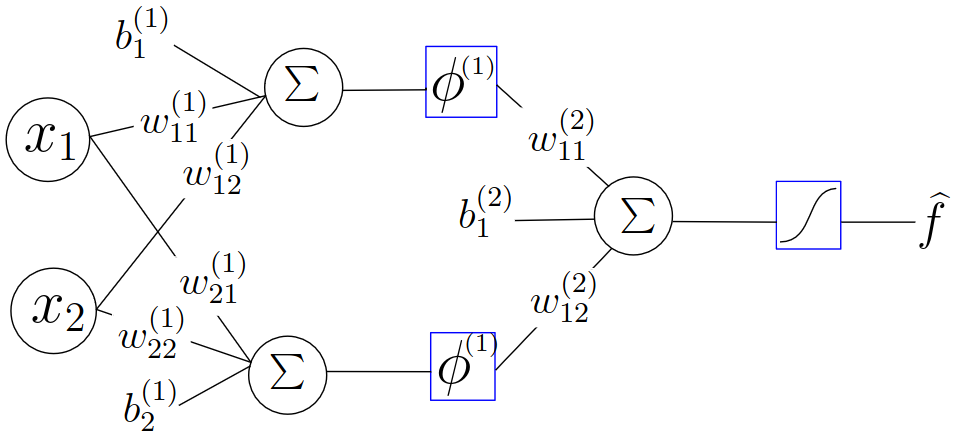
\includegraphics[width=0.8\linewidth]{imgs/neural_net.png}
    \vspace{-3em}
\end{center}

\[
    \bm W^{(1)} = \mattwo{w_{11}^{(1)}}{w_{12}^{(1)}}{w_{21}^{(1)}}{w_{22}^{(1)}} \quad
    \bm b^{(1)} = \cvec{b_1^{(1)}}{b_2^{(1)}} \quad
    \bm X = \matthreetwo{x_1^{(1)}}{x_2^{(1)}}{\vdots}{\vdots}{x_N^{(1)}}{x_N^{(1)}} \quad
    \hat{\bm F} = \cvec{\hat f^{(1)}}{\vdots}{\hat f^{(N)}}
\]
\[
    \bm H^{(i)} = \phi^{(i)}(\bm H^{(i - 1)}{\bm W^{(i)}}^T + \bm b^{(i)}) \qquad \hat{\bm F} = \sigma(\bm H^{(N - 1)}{\bm W^{(N)}}^T + \bm b^{(N)})
\]

\textbf{Logistic sigmoid:} for binary classification: \(\sigma(z) = \frac{1}{1 + e^{-z}}\)\\
\textbf{Softmax:} for multi-class classification: \(\on{softmax}(\bm z) = \frac{e^{z_j}}{\sum _k e_{z_k}}\)

\(\on{logsumexp}(\bm z) = \log\left(\sum _{i} e^{z_i}\right) \implies 
\log\on{softmax}(\bm z)_j = z_j - \on{logsumexp}(\bm z)\)

\textbf{Classification dataset likelihoods:}\\
Binary: i.i.d. Bernoulli, \(\Pr(y | \bm x, \bm w) = \hat f(\bm x; \bm w)^y(1 - \hat f(\bm x; \bm w))^{1 - y}\)
\[
    \hat{\bm w} = \argmax _{\bm w} \sum _{i = 1}^N y^{(i)}\log f(\bm x^{(i)}; \bm w) + (1 - y^{(i)})\log(1 - f(\bm x^{(i)}; \bm w))
\]
Multiclass: i.i.d. Categorical, \(\Pr(\bm y | \bm x, \bm w) = \prod _{j = 1}^K \hat f_j(\bm x; \bm w)^{y_j}\)
\[
    \hat{\bm w} = \argmax _{\bm w} \sum _{i = 1}^N \sum _{j = 1}^K y_j^{(i)}\log f_j(\bm x^{(i)}; \bm w)
\]

\textbf{Backpropagation:} Each node \(z = f(x_1, \dots, x_N)\) in the computational graph is passed an upstream gradient
\(\pdiff{L}{z}\) (sum of all downstream gradients of the nodes that \(z\) connects to) and computes local gradients
\(\pdiff{z}{x_i}\); pass gradients downstream as \(\pdiff{L}{x_i} = \pdiff{L}{z}\pdiff{z}{x_i}\); full gradient is
obtained when leaf is reached. \(+\): distribute gradients; max/min: route gradient to 1 input; \(\times\): swap
gradients.

\begin{center}
    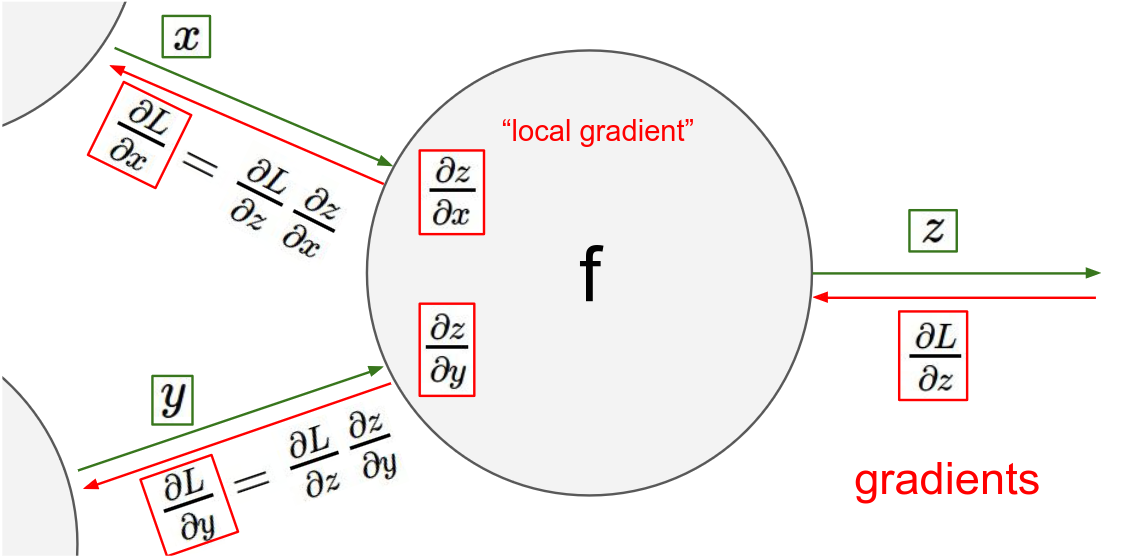
\includegraphics[width=0.8\linewidth]{imgs/backprop.png}
\end{center}

\textbf{Weight initialization:} Aim for zero mean, unit variance of initial hidden states to avoid vanishing or
exploding gradients. \textit{Xavier:} sample from unit Gaussian, divide by square root of number of neuron inputs;
\textit{ReLU:} divide by square root of half the number of inputs.

\subsection{Regularization Techniques}

\textbf{Weight decay:} Equivalent to \(l_2\) regularization; keeps weights small.

\textbf{Early stopping:} Stopping when validation loss increases, before convergence in (training) gradient.

\textbf{Data augmentation:} Creating new samples from existing ones through class-preserving transforms, e.g. rotation,
blurring, cropping, etc. or \textbf{adversarial training} samples designed to mislead the model.

\textbf{Bagging/bootstrap aggregation:} Generate \(k\) datasets of equivalent size from \(\mathcal D\) by sampling with
replacement, and train \(k\) models on datasets; at inference time, average predictions (regression) or vote on class
(classification).

\textbf{Dropout:} During training, drop weights randomly with probability \(1 - \pi\) (typ. \(\pi \in [0.5, 0.8]\)) at
each SGD iteration; during inference, scale weights by \(\pi\). Equivalent to bagging with a \(k\) that increases
exponentially with network size (but same model across all datasets).

\textbf{Weight sharing:} Using prior knowledge to constrain weights to be similar; CNNs are an example.

\subsection{Network Architectures}

\textbf{Convolutional Neural Networks (CNNs):} Convolving 2D (or higher) filters with the input to produce output for
the next layer, keeping structure. Use on highly structured data, e.g. images. Pooling layers between convolutional
layers perform spacial downsampling (but keeps depth). Layers will learn progressively higher-level features until
linearly separable data at the last layer (or passed to MLP).

\textbf{Autoencoders:} Unsupervised model consisting of an encoder from high-dimensional input space to low-dimensional
feature space, and a decoder from feature space back to output space. During training the model is made to reconstruct
its input. Can be used for dimensionality reduction, new sample generation, noise filtering, anomaly detection, etc. or
trained further on labelled data for final task (semi-supervised learning).

\hrulefill
\section{Bayesian Inference} %%%%%%%%%%%%%%%%%%%%%%%%%%%%%%%%%%%%%%%%%%%%%%%%

Given the \textbf{likelihood} \(p(y^{(1)}, \dots, y^{(N)} | \theta) = p(\mathcal D | \theta)\) and the \textbf{prior
distribution} \(p(\theta)\), we wish to find:
\begin{enumerate}
    \item \textbf{Posterior distribution:} \(\displaystyle p(\theta | \mathcal D) = \frac{p(\mathcal D | \theta)p(\theta)}{\int p(\mathcal D | \theta')p(\theta')\,\dtheta'}\)
    \item \textbf{Posterior predictive distribution:} \(\displaystyle p(y' | \mathcal D) = \int p(y' | \theta)p(\theta | \mathcal D)\,\dtheta\)
\end{enumerate}

\textbf{Conjugate prior:} A prior with similar mathematical form as the likelihood; e.g. beta for Bernoulli/geometric,
Gaussian for Gaussian, Dirichlet for multinomial, gamma for Poisson/exponential.

\textbf{Evidence/marginal likelihood:} Likelihood of observing the data when marginalizing across all possible
parameters \(\bm w\) according to the prior:
\begin{align*}
    p(\bm y | \bm X) &= \int p(\bm y | \bm w, \bm X)p(\bm w)\,\dd\bm w \\
    p(\bm y | \bm X, \alpha, \sigma^2) &= \int p(\bm y | \bm w, \bm X, \sigma^2)p(\bm w | \alpha)\,\dd\bm w
\end{align*}

\subsection{Bayesian Linear Regression}

Given dataset \(\mathcal D = \set{(\bm x^{(i)}, y^{(i)})}_{i = 1}^N\), assume \(y \sim \mathcal N(y | \bm w^T\phi(\bm x), \sigma^2)\)
giving likelihood \(\log p(\bm y | \bm w, \bm X, \sigma^2) = \sum _{i = 1}^N \log\mathcal N(y^{(i)} | \bm w^T\bm\phi(\bm x^{(i)}), \sigma^2)\),
with prior \(p(\bm w | \alpha) = \mathcal N(\bm w | \bm 0, \alpha\bm 1)\), Bayesian linear regression gives:
\begin{itemize}
    \item Weight Posterior: \(p(\bm w | \mathcal D) = \mathcal N(\bm w | \bm \mu, \bm\Sigma)\)
    \item Posterior predictive: \(p(y' | \bm x', \mathcal D) = \mathcal N(y' | \bm\mu^T\bm\phi(\bm x'), \bm\phi(\bm x')^T\bm\Sigma\bm\phi(\bm x') + \sigma^2)\)
          where \[\bm\mu = \frac{1}{\sigma^2}\bm\Sigma\bm\phi^T y \qquad \bm\Sigma = \left(\frac{1}{\sigma^2}\bm\Phi^T\bm\Phi + \frac{1}{\alpha}\bm 1\right)^{-1}\]
\end{itemize}

\textbf{Complexity}: \(\mathcal O(NM^2 + M^3)\) time, \(\mathcal O(NM + M^2)\) memory.

\textbf{Type-II inference:} Estimate \(\sigma^2\) and \(\alpha\) through numerical maximization of the (log) 
evidence/marginal likelihood (where \(N\) is number of samples):
\begin{align*}
    \log p(\bm y | \bm X, \alpha, \sigma^2)
    = &-\frac{N}{2}\log\alpha - \frac{N}{2}\log(\sigma^2) - \frac{1}{2\sigma^2}\bm y^T\bm y \\
    &+ \frac{1}{2}\bm\mu^T\bm\Sigma^{-1}\bm\mu + \frac{1}{2}\log\det(\bm\Sigma) - \frac{N}{2}\log(2\pi)
\end{align*}

\subsection{Gaussian Processes}

Define: \textbf{Gram matrix} \(\bm K_{\bm X, \bm X} = \alpha\bm\Phi\bm\Phi^T \in \reals^{N \times N}\), where entry \(ij\) is
\([\bm K_{\bm X, \bm X}]_{ij} = \alpha\bm\phi^T(\bm x^{(i)})\bm\phi(\bm x^{(j)}) = k(\bm x^{(i)}, \bm x^{(j)})\);
\(k \colon \mathcal X \times \mathcal X \mapsto \reals\) is the \textbf{kernel}.
Let \(\bm k_{\bm X, \bm x'} = \rvec{k(\bm x^{(1)}, \bm x')}{k(\bm x^{(2)}, \bm x')}{\dots}{k(\bm x^{(N)}, \bm x')}^T\).
Then the kernelized posterior predictive is
\begin{gather*}
    p(y' | \bm x', \mathcal D) = \mathcal N(y' | \mu _p, \sigma _p^2)
    \qquad \mu _p = \bm k_{\bm x', \bm X}(\bm K_{\bm X, \bm X} + \sigma^2\bm 1)^{-1}\bm y \\
    \sigma _p^2 = k(\bm x', \bm x') - \bm k_{\bm x', \bm X}(\bm K_{\bm X, \bm X} + \sigma^2\bm 1)^{-1}\bm k_{\bm X, \bm x'} + \sigma^2 \\
    \cov(y_1', y_2') = k(\bm x_1', \bm x_2') - \bm k_{\bm x_1', \bm X}(\bm K_{\bm X, \bm X} + \sigma^2\bm 1)^{-1}\bm k_{\bm X, \bm x_2'} + \sigma^2
\end{gather*}
which is equivalent to a GLM with \(l_2\) error and regularization, \(\lambda = \sigma^2/\alpha\).

\(k(\cdot, \cdot)\) specifies covariance between two observations; any collection of observations are jointly Gaussian,
making this a \textbf{Gaussian process}.

\textbf{Complexity:} \(\mathcal O(N^3)\) time, \(\mathcal O(N^2)\) memory. Much more efficient than normal Bayesian
linear regression when \(M \gg N\) or possibly infinite (same kernels as GLMs).

\textbf{Combining kernels:} Through summation \(k(x, y) = k_1(x, y) + k_2(x, y)\) or \(k(\bm x, \bm y) = k_1(x_1, y_1) +
k_2(x_2, y_2)\), multiplication \(k(x, y) = k_1(x, y)k_2(x, y)\) or \(k(\bm x, \bm y) = k_1(x_1, y_1)k_2(x_2, y_2)\), or
composition \(k(x, y) = k_1(f(x), f(y))\), all preserving positive-definiteness.

\textbf{Type-II inference:} In function-space,
\[\begin{split}
    \log p(\bm y | \bm X, \alpha, \sigma^2) = &-\frac{N}{2}\log(2\pi) - \frac{1}{2}\log\det(\bm K_{\bm X, \bm X} + \sigma^2\bm 1) \\
    &-\frac{1}{2}\bm y^T(\bm K_{\bm X, \bm X} + \sigma^2\bm 1)^{-1}\bm y
\end{split}\]

\subsection{Approximate Bayesian Inference}

Given observed evidence, \(X_E\) and unobserved variables, \(X_F\), find
\[p(X_F | X_E) = \frac{p(X_E, X_F)}{p(X_E)}\]
\(p(X_E, X_F) = p(X_E | X_F)p(X_F)\) is often known from the model and prior assumptions,
but \(p(X_E) = \int p(X_E, X_F)\,\dd X_F\) is intractable to compute.

\textbf{Quadrature:} Numerically integrate \(p(X_E) = \int p(X_E, X_F)\,\dd X_F\) by sampling a finite number of points.
Infeasible due to the exponential growth in points required. Error usually scales as \(\mathcal O(n^{-\frac{1}{d}})\)
where \(d\) is the dimensionality of the integral. Beyond \(d \geq 3\) Monte Carlo is better.

\textbf{Laplace approximation:} Let \(X_F = \bm z\) and \(\hat{\bm z}_\text{MAP} = \argmax _{\bm z} \log\tilde p(\bm z)\)
where \(\tilde p(\bm z) = p(X_E, \bm z)\), then \(p(\bm z | X_E) = \frac{1}{Z}p(X_E, \bm z) = \frac{1}{Z}\tilde p(\bm z)\).
Then:
\[
    p(\bm z | X_E) \approx \mathcal N(\bm z | \hat{\bm z}_\text{MAP}, \bm A^{-1})
    \qquad \eval{\bm A = -\del^2\log\tilde p(\bm z)}{\bm z = \hat{\bm z}_\text{MAP}}
\]
Note: from a second-order Taylor expansion:
\[
    \log p(\bm z | X_E) \approx \log \tilde p(\hat{\bm z}_\text{MAP})
    - \frac{1}{2}(\bm z - \hat{\bm z}_\text{MAP})^T\bm A(\bm z - \hat{\bm z}_\text{MAP}) + \text{const.}
\]
Simple but poor performance, since it does not account for global information.
However, if posterior is Gaussian, this is exact.
Requires existence of Hessian for likelihood and prior, so certain distributions (e.g. Laplace) might be bad.
    
\subsubsection{Stochastic Variational Inference (SVI)}

\textbf{Kullback-Leibler (KL) divergence:} For two distributions \(p(\bm z)\) and \(q(\bm z)\),
\[
    KL\infdivx{q}{p} = \mathbb E_{\bm z \sim q(\bm z)}\left[\log\frac{q(\bm z)}{p(\bm z)}\right]
    \implies \begin{cases}
        KL\infdivx{q}{p} \geq 0 \\
        KL\infdivx{q}{p} = 0 \iff q = p \\
        KL\infdivx{q}{p} \neq KL\infdivx{p}{q} \\
    \end{cases}
\]
\textit{Reverse-KL (information projection):} take \(KL\infdivx{q}{p}\) which penalizes \(q\) having mass where \(p\)
has none (compressing \(q\) to fit to one peak of \(p\)); \textit{forward-KL (moment projection):} take
\(KL\infdivx{p}{q}\) which penalizes \(q\) missing mass where \(p\) has mass (stretching out \(q\) to cover all peaks of
\(p\)). Reverse KL commonly used for computational reasons.

\textbf{Stochastic Variational Inference (SVI):} Approximating the true conditional \(p(\bm z | \bm x) = \frac{p(\bm x, \bm z)}{p(\bm x)}\)
by a simpler distribution, \(q(\bm z | \bm \theta)\), from a known family of distributions, such that
\(KL\infdivx{q(\bm z | \bm\theta)}{p(\bm z | \bm x)}\) is minimized.

\textbf{Evidence lower bound (ELBO):} \(\mathcal L(\bm\theta, \bm x) = -\expectation{\bm z \sim q}{\log\frac{q(\bm z | \bm\theta)}{p(\bm z, \bm x)}}\)
is a lower bound for \(\log p(\bm x)\); maximizing ELBO minimizes KL.
Has gradient
\[
    \del _{\bm\theta}\mathcal L(\bm\theta, \bm x) = \del _{\bm\theta}\int q(\bm z | \bm\theta)\log\frac{p(\bm x, \bm z)}{q(\bm z | \bm \theta)}\,\dd\bm z
\]

\textbf{Score function/REINFORCE gradient estimator:} By Monte Carlo:
\begin{align*}
    \del _{\bm\theta}\mathcal L(\bm\theta, \bm x)
    &= \expectation{\bm z \sim q}{\del _{\bm\theta} \log q(\bm z | \bm\theta)\log\frac{p(\bm x, \bm z)}{q(\bm z | \bm\theta)}} \\
    &\approx \frac{1}{B}\sum _{i = 1}^B \del _{\bm\theta}\log q(\bm z^{(i)} | \bm\theta)\log\frac{p(\bm x, \bm z^{(i)})}{q(\bm z^{(i)} | \bm\theta)}
\end{align*}

\textbf{Pathwise/reparametrization gradient estimator:} Find \(T(\bm\varepsilon, \bm\theta)\) such that for
\(\bm\varepsilon \sim p(\bm\varepsilon)\), then \(\bm z = T(\bm\varepsilon, \bm\theta) \implies \bm z \sim q(\bm z | \bm\theta)\).
Then Monte Carlo:
\begin{align*}
    \del _{\bm\theta} \mathcal L(\bm\theta, \bm x)
    &= \expectation{\bm\varepsilon \sim p(\bm\varepsilon)}{\del _{\bm\theta}\log \frac{p(\bm x, T(\bm\varepsilon, \bm\theta))}{q(T(\bm\varepsilon, \bm\theta) | \bm\theta)}} \\
    &\approx \frac{1}{B}\sum _{i = 1}^B \del _{\bm\theta}\log \frac{p(\bm x, T(\bm\varepsilon^{(i)}, \bm\theta))}{q(T(\bm\varepsilon^{(i)}, \bm\theta) | \bm\theta)}
\end{align*}
e.g. for a Gaussian, \(\bm\theta = \set{\mu, \sigma^2}\), let \(\varepsilon \sim \mathcal N(\varepsilon | 0, 1)\) and
\(T(\varepsilon, \bm\theta) = \sigma\varepsilon + \mu\), then \(z \sim \mathcal N(z | \mu, \sigma^2)\).

\subsubsection{Expectation Approximation}

Instead of \(p(\bm x)\) sometimes we only need \(I = \expectation{\bm x \sim p(\bm x)}{\phi(\bm x)}\).

\textbf{Monte Carlo:} Collect \(R\) random samples from \(p(\bm x)\), denoted \(\bm x^{(i)}\), then
\[
    I = \int \phi(\bm x)p(\bm x)\,\dd\bm x \approx \hat I = \frac{1}{R}\sum _{i = 1}^R \phi(\bm x^{(i)})
\] 
Has standard deviation proportional to \(1/\sqrt{R}\), independent of dimension; unbiased estimator.
For dimension \(d \geq 3\) this generally outperforms quadrature.

However, we might only know the unnormalized \(\tilde p(\bm x) = Zp(\bm x)\), or sampling may be difficult due to high
dimensionality, in which case we need importance sampling.

\textbf{Importance Sampling:} Let \(q(\bm x)\) be the \textit{sampler density}, a density easy to sample from; then
for some unnormalized \(\tilde p(\bm x) = Zp(\bm x)\),
\[
    I = \frac{\expectation{\bm x \sim q(\bm x)}{\frac{\phi(\bm x)\tilde p(\bm x)}{q(\bm x)}}}{\expectation{\bm x \sim q(\bm x)}{\frac{\tilde p(\bm x)}{q(\bm x)}}}
    \implies \hat I = \frac{\frac{1}{R}\sum _{r = 1}^R \frac{\phi(\bm x^{(r)})\tilde p(\bm x^{(r)})}{q(\bm x^{(r)})}}{\frac{1}{R}\sum _{r = 1}^R \frac{\tilde p(\bm x^{(r)})}{q(\bm x^{(r)})}} = \frac{\sum _r w_r\phi(\bm x^{(r)})}{\sum _r w_r}
\]
where each \(w_r = \tilde p(\bm x^{(r)}) / q(\bm x^{(r)})\) is an \textit{importance weight}, which is larger if
sampling from \(q(\bm x)\) tends to under-represent the point, or smaller for over-represent.
Note if \(\tilde p(\bm x) = p(\bm x)\) is normalized, then
\[
    \expectation{\bm x \sim q(\bm x)}{\frac{\tilde p(\bm x)}{q(\bm x)}} = 1
    \implies \hat I = \frac{1}{R}\sum _{r = 1}^R \frac{\phi(\bm x^{(r)})\tilde p(\bm x^{(r)})}{q(\bm x^{(r)})}
    = \frac{1}{R}\sum _r w_r\phi(\bm x^{(r)})
\]

Sampler should have heavy tails (e.g. Cauchy instead of Gaussian) to compensate for differences between \(p(\bm x)\) and
\(q(\bm x)\). If the sampler is chosen improperly, the variance of the result can be extremely high. In high dimensions,
if the sampler distribution is not a near-perfect approximation of the target, then the entire sum will likely be
dominated by a few samples with a huge weight, leading to a very bad estimate.

\hrulefill
\section{Useful Identities} %%%%%%%%%%%%%%%%%%%%%%%%%%%%%%%%%%%%%%%%%%%%%%%%

\textbf{Matrix differentiation:} \(\pdiff{}{z}(\bm z^T\bm A\bm z) = (\bm A + \bm A^T)\bm z \qquad \pdiff{}{\bm z}(\bm A\bm z) = \bm A^T\)

\textbf{Laplace distribution:} \(\operatorname{Lap}(\epsilon | \mu, b) = \frac{1}{2b}e^{-\frac{\abs{\epsilon - \mu}}{b}}\)
with \(\sigma^2 = 2b^2\).

\textbf{Gaussian distribution:} \(\mathcal N(x | \mu, \sigma^2) = \frac{1}{\sqrt{2\pi}\sigma}e^{-\frac{1}{2\sigma^2}(x - \mu)^2}\);
multi-var ver.:
\[
    \mathcal N(\bm x | \bm\mu, \bm\Sigma) = \frac{1}{(2\pi)^\frac{n}{2}\det(\bm\Sigma)^\frac{1}{2}}\exp\left[-\frac{1}{2}(\bm x - \bm \mu)^T\bm \Sigma^{-1}(\bm x - \bm \mu)\right]
\]
Partition Gaussian \(\bm x \sim \mathcal N(\bm x | \bm\mu, \bm\Sigma)\) as:
\[\bm x = \cvec{\bm x_1}{\bm x_2}, \bm\mu = \cvec{\bm\mu _1}{\bm\mu _2}, \bm\Sigma = \mattwo{\bm\Sigma _{11}}{\bm\Sigma _{12}}{\bm\Sigma _{21}}{\bm\Sigma _{22}} \implies \bm x \sim f(\bm x_1, \bm x_2)\]
Then \(\bm x_1 \sim \mathcal N(\bm x_1 | \bm\mu _1, \bm\Sigma _{11}), \bm x_2 \sim \mathcal N(\bm x | \bm\mu _2, \bm\Sigma _{22})\), and
\[f(\bm x_1 | \bm x_2) = \mathcal N(\bm x_1 | \bm\mu _1 + \bm\Sigma _{12}\bm\Sigma _{22}^{-1}(\bm x_2 - \bm\mu _2), \bm\sigma _{11} - \bm\Sigma _{12}\bm\Sigma _{22}^{-1}\bm\Sigma _{21})\]

\textbf{Beta distribution:} \(p(\theta | \alpha, \beta) = \frac{\Gamma(\alpha + \beta)}{\Gamma(\alpha)\Gamma(\beta)}\theta^{\alpha - 1}(1 - \theta)^{\beta - 1}\)
(\(\alpha = \beta = 1\) gives uniform dist.) with mean \(\frac{\alpha}{\alpha + \beta}\) and mode
\(\frac{\alpha - 1}{\alpha + \beta - 2}\).

\textbf{Dirichlet distribution:} \(p(\bm\theta | \alpha _1, \dots, \alpha _K) = \frac{\Gamma\left(\sum _k \alpha _k\right)}{\prod _k \Gamma(\alpha _k)}\prod _k \theta _k^{\alpha _k - 1}\) where \(\alpha _k > 0, \sum _k \alpha _k = 1\).

\textbf{Sigmoid \& Derivative:} \(\sigma(x) = \frac{1}{1 + e^{-x}} \implies \diff{}{x}\sigma(x) = \sigma(x)(1 - \sigma(x))\)

\end{document}
